% act_d3_teacher.tex — Iskole: Teacher Workflow
\documentclass[a4paper,landscape]{article}
\usepackage[a4paper,landscape,top=1.8cm,bottom=1.2cm,left=1.2cm,right=1.2cm]{geometry}
\usepackage[dvipsnames,svgnames]{xcolor}
\usepackage{tikz}
\usetikzlibrary{shapes.geometric,arrows.meta,calc}
\usepackage{fancyhdr}
\definecolor{ColHdr} {RGB}{30,58,138}
\definecolor{ActFill}{RGB}{219,234,254}
\definecolor{ActLine}{RGB}{52,109,219}
\definecolor{SysFill}{RGB}{220,254,220}
\definecolor{SysLine}{RGB}{34,139,34}
\definecolor{SwimBg} {RGB}{240,240,248}
\tikzset{
  nd_start/.style={circle,fill=black,minimum size=10pt,inner sep=0pt},
  nd_stop/.style={circle,fill=black,draw=black,double,double distance=2pt,minimum size=10pt,inner sep=0pt},
  nd_act/.style={rectangle,rounded corners=3pt,draw=ActLine,fill=ActFill,text width=4.9cm,minimum height=0.62cm,align=center,font=\footnotesize},
  nd_sys/.style={rectangle,rounded corners=3pt,draw=SysLine,fill=SysFill,text width=4.9cm,minimum height=0.62cm,align=center,font=\footnotesize\itshape},
  arr/.style={-{Stealth[length=5pt,width=4pt]},thick},
}
\newcommand{\swimbox}[4]{%
  \fill[SwimBg,rounded corners=4pt](#1-2.6,#2+0.15) rectangle (#1+2.6,#3);
  \node[font=\small\bfseries\color{ColHdr}] at (#1,#2) {#4};}
\pagestyle{fancy}\fancyhf{}
\fancyhead[C]{\bfseries\color{ColHdr}Iskole — Activity Diagram 3: Teacher Workflow}
\fancyfoot[C]{\small\thepage}
\renewcommand{\headrulewidth}{1pt}
\renewcommand{\headrule}{\hbox to\headwidth{\color{ColHdr}\leaders\hrule height 1pt\hfill}}
\setlength{\headheight}{16pt}
\begin{document}
\begin{center}
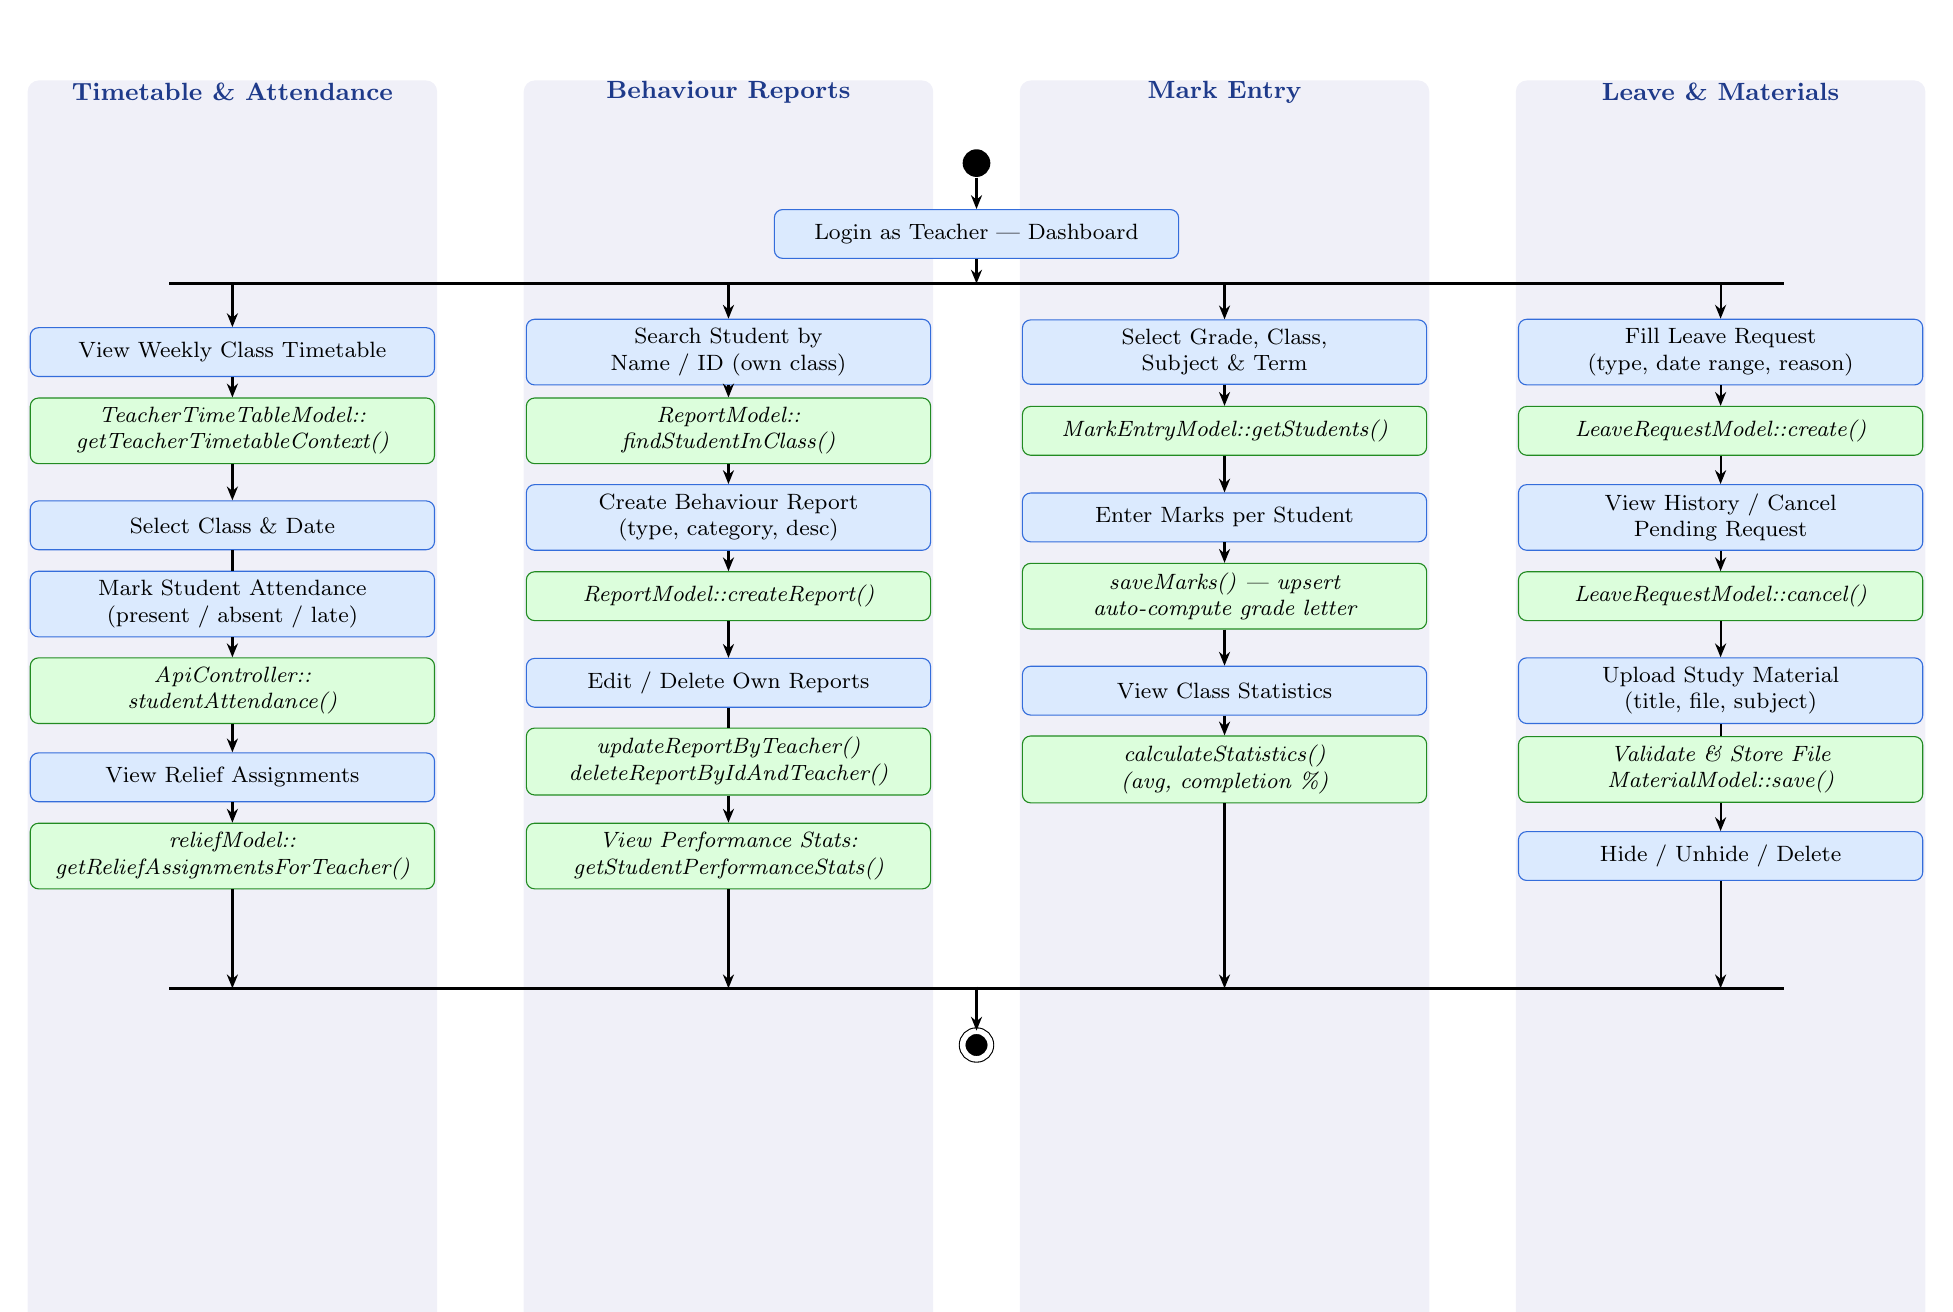
\begin{tikzpicture}[x=1cm,y=1cm]
\def\cA{3.3}\def\cB{9.6}\def\cC{15.9}\def\cD{22.2}
\swimbox{\cA}{0.2}{-15.5}{Timetable \& Attendance}
\swimbox{\cB}{0.2}{-15.5}{Behaviour Reports}
\swimbox{\cC}{0.2}{-15.5}{Mark Entry}
\swimbox{\cD}{0.2}{-15.5}{Leave \& Materials}
\node[nd_start] at (12.75,-0.7)(S){};
\node[nd_act]   at (12.75,-1.6)(HD){Login as Teacher \textemdash{} Dashboard};
\fill[black](2.5,-2.25) rectangle (23.0,-2.21);
% Col A
\node[nd_act] at (\cA,-3.1)(A1){View Weekly Class Timetable};
\node[nd_sys] at (\cA,-4.1)(A2){TeacherTimeTableModel::\\getTeacherTimetableContext()};
\node[nd_act] at (\cA,-5.3)(A3){Select Class \& Date};
\node[nd_act] at (\cA,-6.3)(A4){Mark Student Attendance\\(present / absent / late)};
\node[nd_sys] at (\cA,-7.4)(A5){ApiController::\\studentAttendance()};
\node[nd_act] at (\cA,-8.5)(A6){View Relief Assignments};
\node[nd_sys] at (\cA,-9.5)(A7){reliefModel::\\getReliefAssignmentsForTeacher()};
% Col B
\node[nd_act] at (\cB,-3.1)(B1){Search Student by\\Name / ID (own class)};
\node[nd_sys] at (\cB,-4.1)(B2){ReportModel::\\findStudentInClass()};
\node[nd_act] at (\cB,-5.2)(B3){Create Behaviour Report\\(type, category, desc)};
\node[nd_sys] at (\cB,-6.2)(B4){ReportModel::createReport()};
\node[nd_act] at (\cB,-7.3)(B5){Edit / Delete Own Reports};
\node[nd_sys] at (\cB,-8.3)(B6){updateReportByTeacher()\\deleteReportByIdAndTeacher()};
\node[nd_sys] at (\cB,-9.5)(B7){View Performance Stats:\\getStudentPerformanceStats()};
% Col C
\node[nd_act] at (\cC,-3.1)(C1){Select Grade, Class,\\Subject \& Term};
\node[nd_sys] at (\cC,-4.1)(C2){MarkEntryModel::getStudents()};
\node[nd_act] at (\cC,-5.2)(C3){Enter Marks per Student};
\node[nd_sys] at (\cC,-6.2)(C4){saveMarks() \textemdash{} upsert\\auto-compute grade letter};
\node[nd_act] at (\cC,-7.4)(C5){View Class Statistics};
\node[nd_sys] at (\cC,-8.4)(C6){calculateStatistics()\\(avg, completion \%)};
% Col D
\node[nd_act] at (\cD,-3.1)(D1){Fill Leave Request\\(type, date range, reason)};
\node[nd_sys] at (\cD,-4.1)(D2){LeaveRequestModel::create()};
\node[nd_act] at (\cD,-5.2)(D3){View History / Cancel\\Pending Request};
\node[nd_sys] at (\cD,-6.2)(D4){LeaveRequestModel::cancel()};
\node[nd_act] at (\cD,-7.4)(D5){Upload Study Material\\(title, file, subject)};
\node[nd_sys] at (\cD,-8.4)(D6){Validate \& Store File\\MaterialModel::save()};
\node[nd_act] at (\cD,-9.5)(D7){Hide / Unhide / Delete};
% join
\fill[black](2.5,-11.2) rectangle (23.0,-11.16);
\node[nd_stop] at (12.75,-11.9)(E){};
% arrows
\draw[arr](S)--(HD);
\draw[arr](HD.south)--(12.75,-2.23);
\foreach \x/\n in {\cA/A1,\cB/B1,\cC/C1,\cD/D1}{\draw[arr](\x,-2.23)--(\n);}
\draw[arr](A1)--(A2);\draw[arr](A3)--(A4)--(A5);\draw[arr](A6)--(A7);\draw[arr](A2)--(A3);\draw[arr](A5)--(A6);
\draw[arr](B1)--(B2);\draw[arr](B3)--(B4);\draw[arr](B5)--(B6)--(B7);\draw[arr](B2)--(B3);\draw[arr](B4)--(B5);
\draw[arr](C1)--(C2);\draw[arr](C3)--(C4);\draw[arr](C5)--(C6);\draw[arr](C2)--(C3);\draw[arr](C4)--(C5);
\draw[arr](D1)--(D2);\draw[arr](D3)--(D4);\draw[arr](D5)--(D6)--(D7);\draw[arr](D2)--(D3);\draw[arr](D4)--(D5);
\draw[arr](A7)--(\cA,-11.18);
\draw[arr](B7)--(\cB,-11.18);
\draw[arr](C6)--(\cC,-11.18);
\draw[arr](D7)--(\cD,-11.18);
\draw[arr](12.75,-11.16)--(E);
\end{tikzpicture}
\end{center}
\end{document}
